\rhead{\textit{Problem design}}
\lhead{}
\subsection{Interaction Metaphors}
\subsubsection{Deaf person}
\begin{table}[h]
	\begin{tabular}{|l|l|l|}
		\hline
		\multicolumn{1}{|r|}{Activity}                                                                              & Real World Metaphore & \multicolumn{1}{r|}{Implications for Activities}                                                                                      \\ \hline
		\begin{tabular}[c]{@{}l@{}}Being able to remember the gestures\\  of every single word is like\end{tabular} & A filing cabinet     & \begin{tabular}[c]{@{}l@{}}- Word list \\- Search key\end{tabular} \\ \hline
		\begin{tabular}[c]{@{}l@{}}Having a report on your improvements \\ is like\end{tabular}                     & An agenda            & \begin{tabular}[c]{@{}l@{}}- List of learned words\\
			- Key to see gestures of learned words\end{tabular}                                \\ \hline
		\begin{tabular}[c]{@{}l@{}}Be able to video call friends to test \\ your own improvements\end{tabular}      & A telephone          & \begin{tabular}[c]{@{}l@{}}- Friends list\\
			- Button for video calling a friend \end{tabular}                                               \\ \hline
	\end{tabular}
\end{table}
\subsubsection{Family and friends}
\begin{table}[h]
	\begin{tabular}{|l|l|l|}
		\hline
		\multicolumn{1}{|r|}{Activity}                                                        & \multicolumn{1}{r|}{Real World Metaphore} & Implications for Activities                                                                              \\ \hline
		\begin{tabular}[c]{@{}l@{}}Receive immediate feedback\\ on self-learning\end{tabular} & A messaging system                        & \begin{tabular}[c]{@{}l@{}}- Friends list\\ - Button for video calling a friend\end{tabular}             \\ \hline
		Display all word learned                                                              & A diary                                   & \begin{tabular}[c]{@{}l@{}}- List of learned words\\ - Key to see gestures of learned words\end{tabular} \\ \hline
	\end{tabular}
\end{table}
\clearpage
\subsection{Interaction Sketch}
\subsubsection{Deaf person}
\begin{figure}[h]
	\centering
	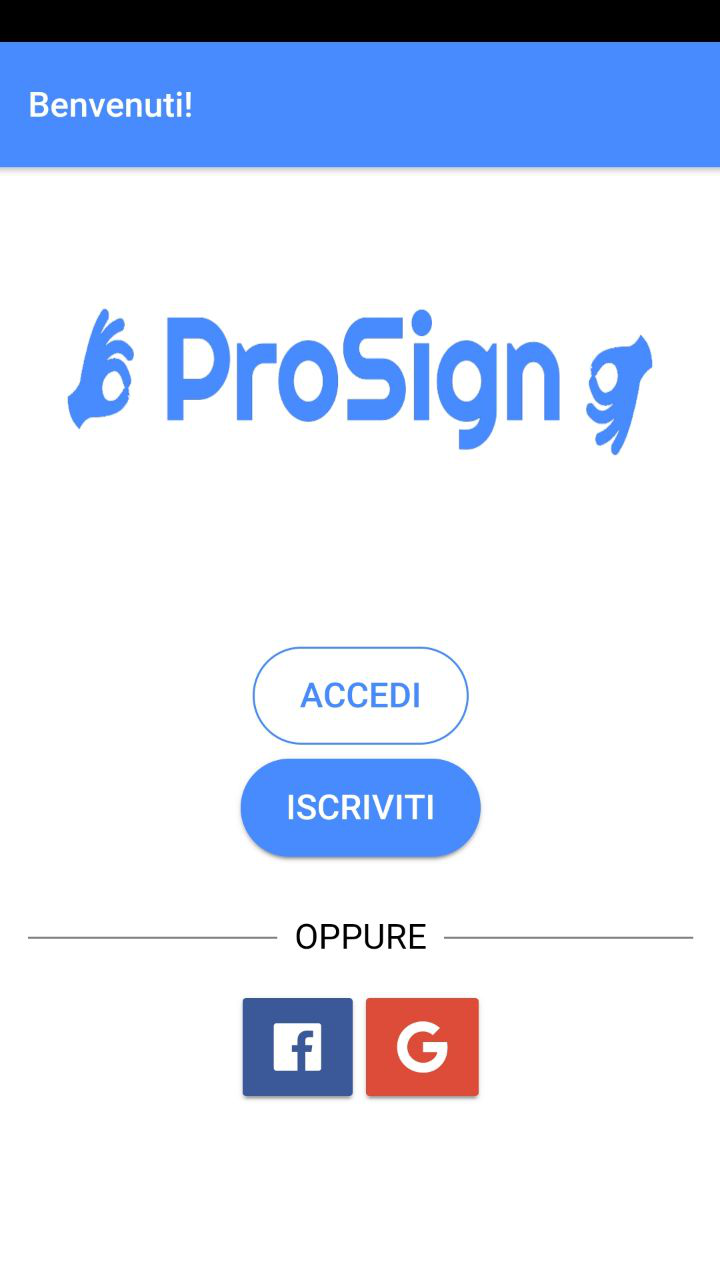
\includegraphics[width=0.25\linewidth]{Figure/screenshot001}
	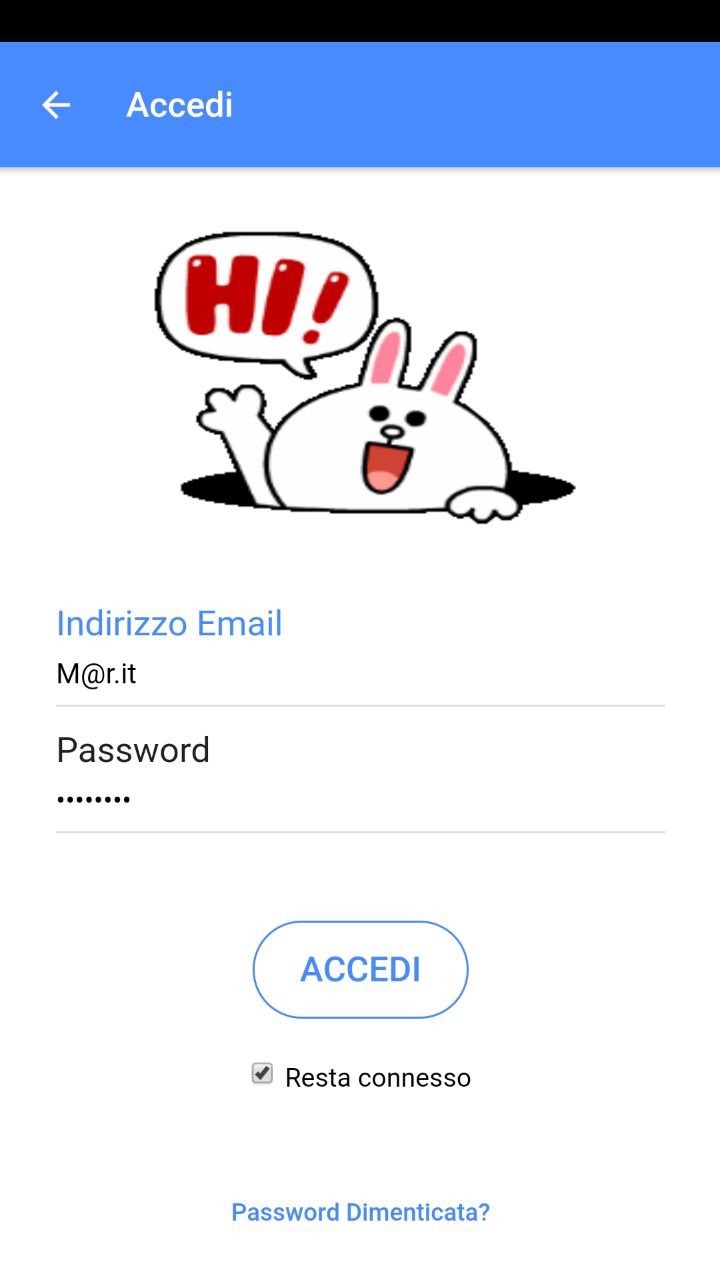
\includegraphics[width=0.25\linewidth]{Figure/screenshot002}
	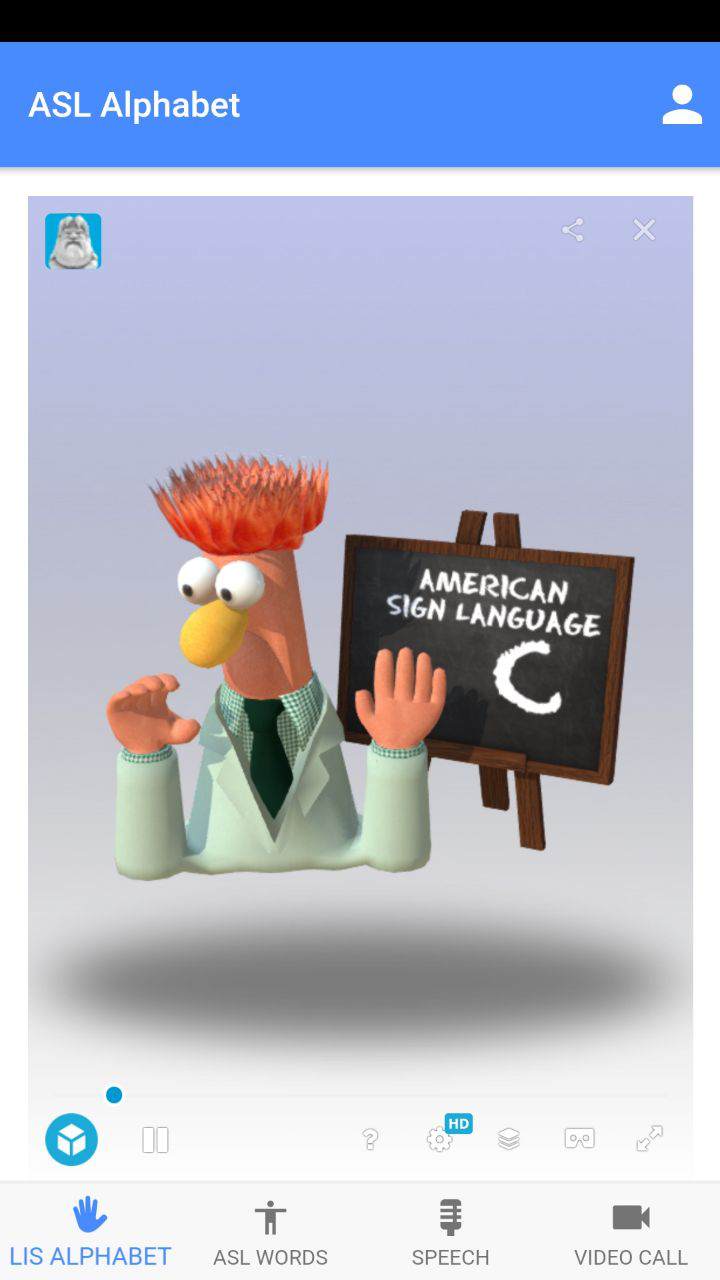
\includegraphics[width=0.25\linewidth]{Figure/screenshot003}
	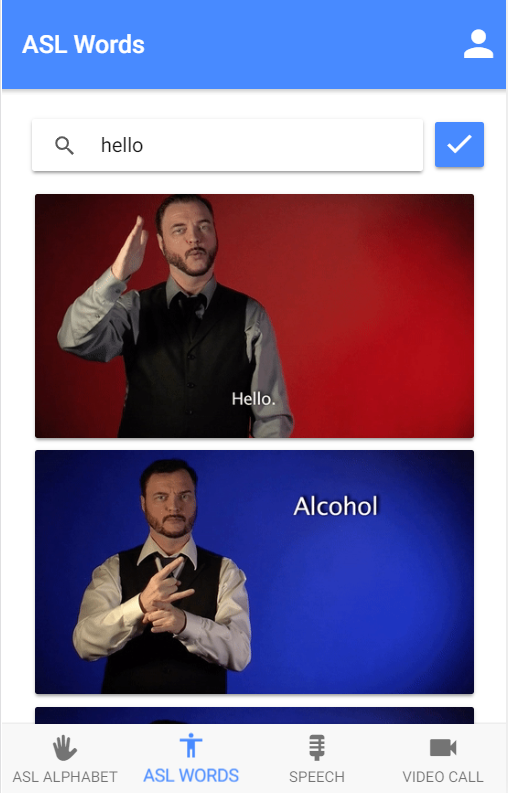
\includegraphics[width=0.25\linewidth]{Figure/ASLWORDSPAGE}
	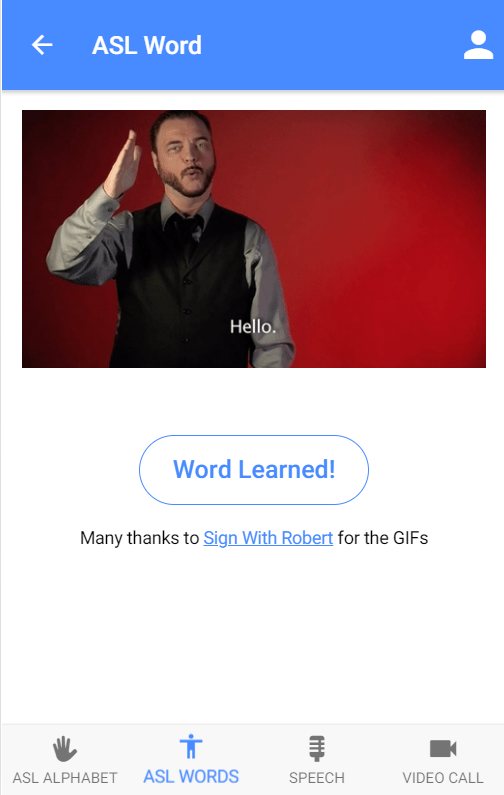
\includegraphics[width=0.25\linewidth]{Figure/ASLWORDPAGE}
	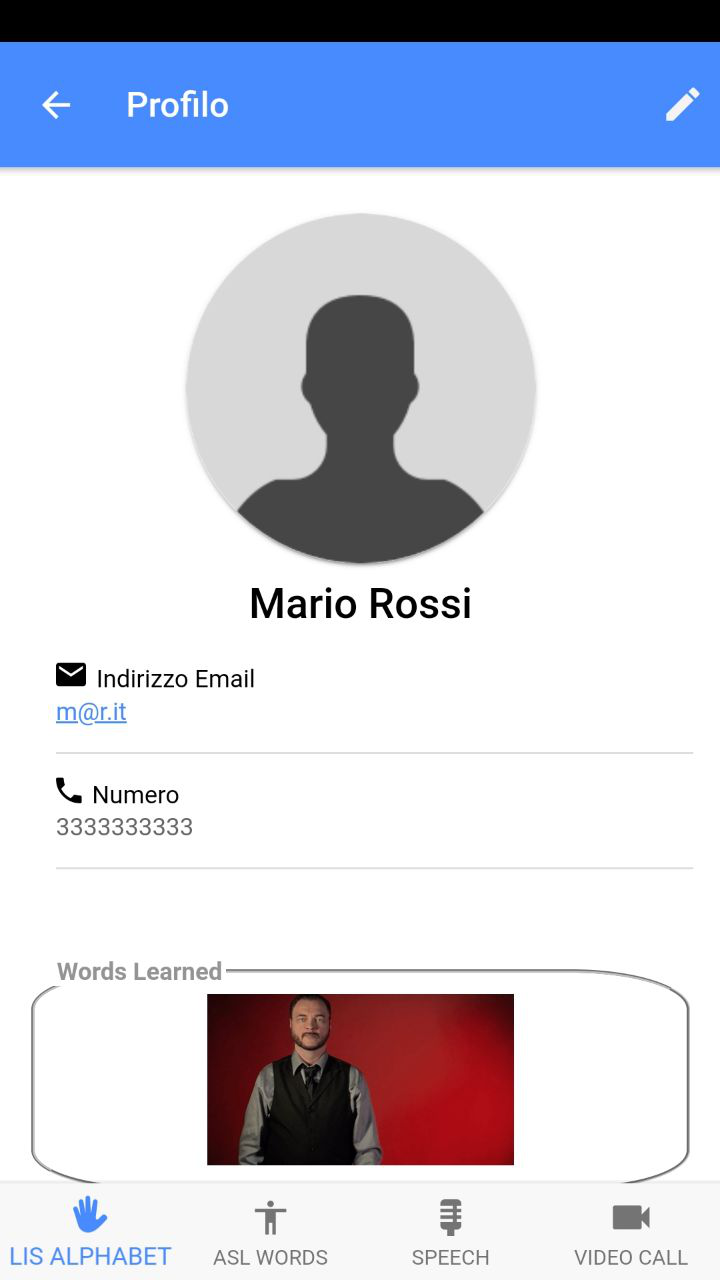
\includegraphics[width=0.25\linewidth]{Figure/screenshot004}
	\label{fig:screenshot004}
\end{figure}
\clearpage
\subsubsection{Family and friends}
\begin{figure}[h]
	\centering
	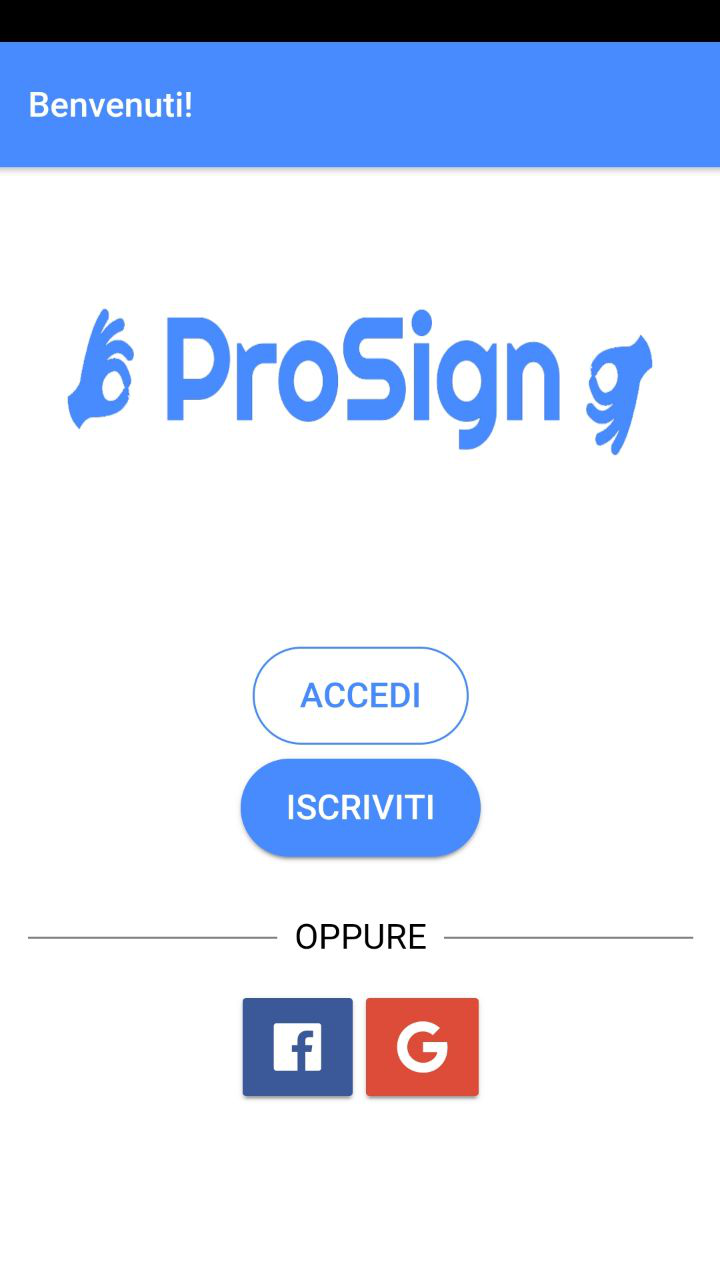
\includegraphics[width=0.25\linewidth]{Figure/screenshot001}
	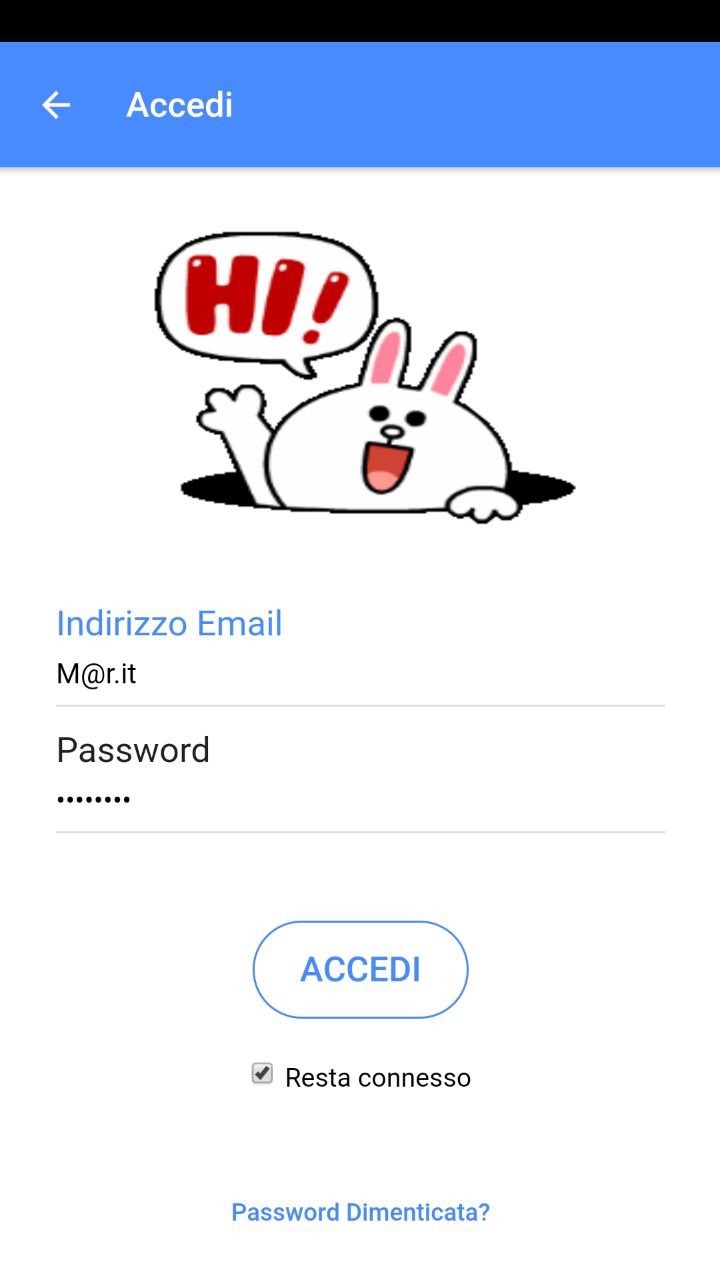
\includegraphics[width=0.25\linewidth]{Figure/screenshot002}
	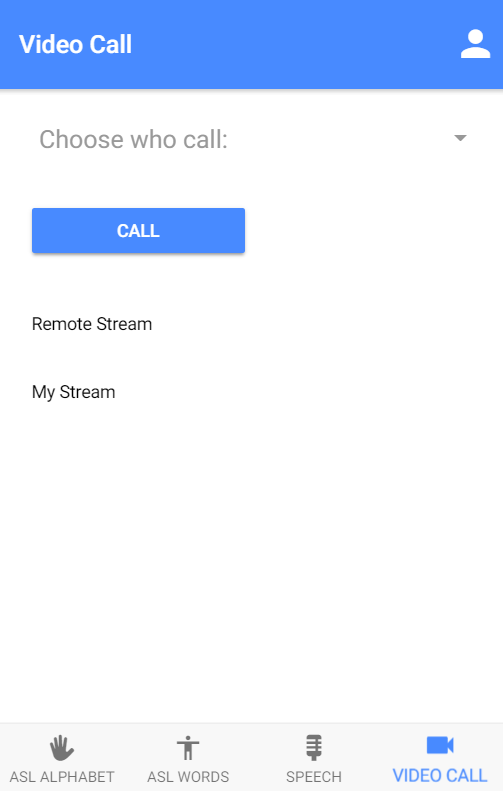
\includegraphics[width=0.3\linewidth]{Figure/screenshot006}
	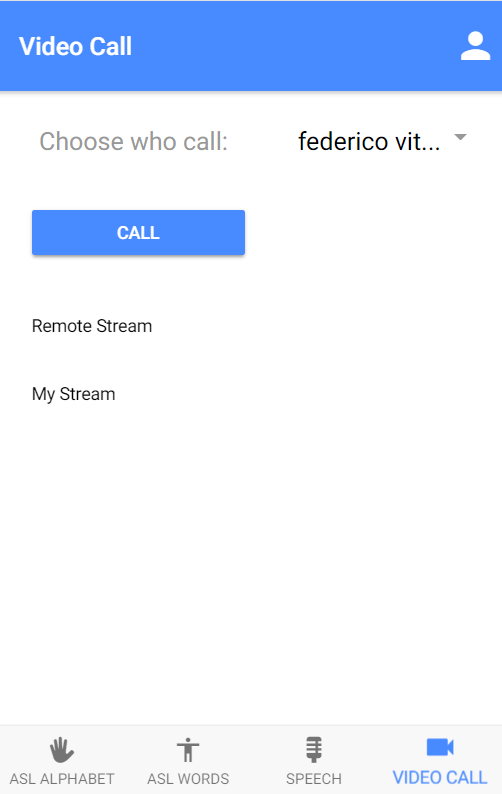
\includegraphics[width=0.25\linewidth]{Figure/screenshot007}
	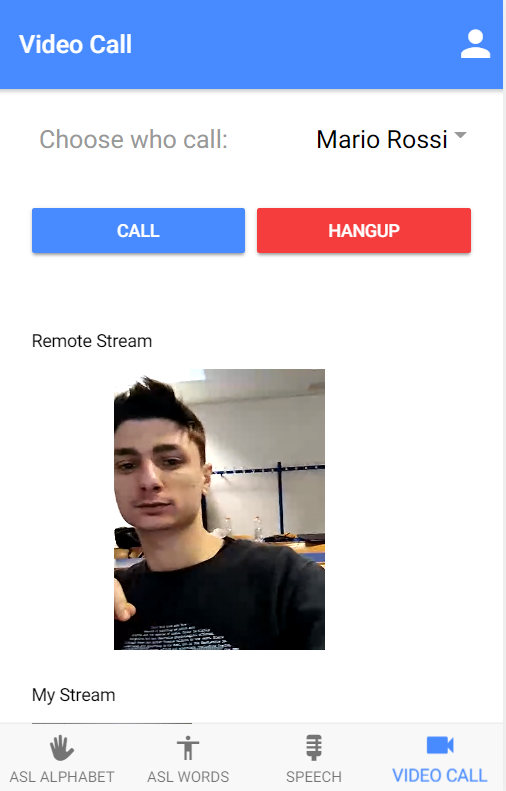
\includegraphics[width=0.25\linewidth]{Figure/screenshot005}
\end{figure}


\subsection{Interaction Scenarious}
\subsubsection{Deaf person}
\begin{itemize}
	\item Mario wants to learn new words
	\item Mario accesses the app
	\item He goes to the section containing the list of words
	\item Using the appropriate button, search for the desired word
	\item Learn gestures
	\item Mark the word as learned
	\item Mario logs out
\end{itemize}
\subsubsection{Family and friends}
\begin{itemize}
	\item Luca wants to video call a friend to show his improvements
	\item Luca accesses the app
	\item He goes to the section that allows video calls
	\item Using the appropriate button select the friend to call and start the call
	\item Once the call is initiated, it shows him all its improvements
	\item Luca greets his friend and stops the call
	\item Luca logs out
\end{itemize}

\clearpage
\subsection{Conceptual model}
\begin{figure}[h]
	\centering
	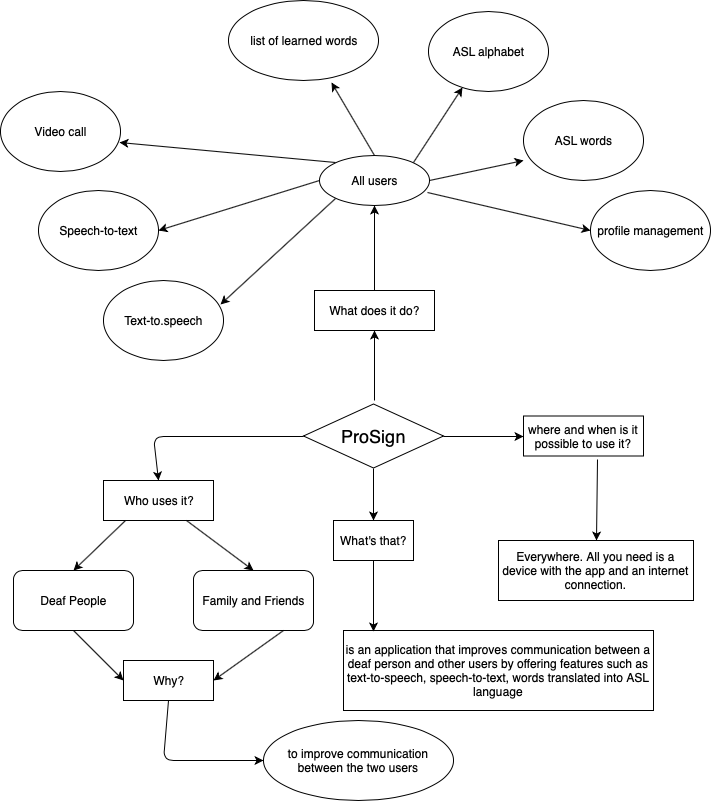
\includegraphics[width=0.7\linewidth]{Figure/screenshot008}
\end{figure}
